\documentclass[12pt,a4paper,oneside]{report}
\usepackage[OT1]{fontenc}
\renewcommand{\rmdefault}{ptm}
\usepackage{amsmath,amssymb,booktabs,multirow,graphicx,subcaption,url,xcolor,threeparttable}
\usepackage[hidelinks]{hyperref}
\setlength{\textwidth}{155mm}
\setlength{\textheight}{230mm}
\setlength{\oddsidemargin}{4.6mm}
\setlength{\evensidemargin}{4.6mm}
\setlength{\topmargin}{-10mm}
\linespread{1.25}
\setlength{\emergencystretch}{3em}
\graphicspath{{../figures/}}
\newcommand{\AUC}{\operatorname{AUC}}
\newcommand{\EER}{\operatorname{EER}}
\newcommand{\TAR}{\operatorname{TAR}}
\newcommand{\FAR}{\operatorname{FAR}}
\begin{document}
\hypersetup{pageanchor=false}
\begin{titlepage}
\centering
\vspace*{12mm}
{\Large Research Thesis Draft\par}
\vspace{15mm}
{\LARGE Parameter-Efficient Periocular Fusion for Cross-Condition and Cross-Dataset Occlusion-Robust Face Verification\par}
\vspace{20mm}
{\Large Pararajasingham Sangiya\par}
\vspace{5mm}
Independent Researcher\par
ORCID: 0009-0005-3407-2154\par
\vfill
Prepared for author review\par
15 November 2026\par
\vspace{12mm}
\raggedright
This report presents the completed research in an extended thesis format. It is not an institution-approved thesis or a record of submission. No university, degree, supervisor, ethics approval, or examination outcome is asserted. Institution-specific front matter and formatting must be supplied before an academic submission.
\end{titlepage}
\pagenumbering{roman}
\hypersetup{pageanchor=true}
\chapter*{Abstract}
\addcontentsline{toc}{chapter}{Abstract}
Masks and sunglasses remove different sources of facial identity information, making it unclear when a periocular representation should complement a whole-face model. We study this question using DINOv2, low-rank adaptation (LoRA), and five configurations ranging from a frozen encoder with a trained projection to dual-branch learned fusion. Fifteen models are trained for five complete epochs on CPU using three seeds and a 6,171-image ROF manifest that excludes known content conflicts. Periocular LoRA achieves the highest masked ROC-AUC (0.9221$\pm$0.0046), fixed fusion leads on sunglasses (0.8950$\pm$0.0021), and learned fusion leads on neutral faces (0.9458$\pm$0.0026). After excluding a known training-name overlap, learned fusion achieves 0.9548$\pm$0.0022 on 802 MFR2 pairs. Fixed fusion leads on 21,798 exact-conflict-excluded RMFRD pairs (0.7240$\pm$0.0099). Controls that retain the same trained branches show that image-dependent gate weights do not consistently improve on constant weights. Validation-calibrated thresholds also reveal false-accept shifts that retrospective ROC summaries conceal. A separate SFace diagnostic achieves higher AUC under different pretraining and alignment. The results support condition-dependent regional complementarity, while showing why neither the presence of a learned gate nor a high AUC alone establishes reliable verification under occlusion.

\chapter*{Reader's Guide}
\addcontentsline{toc}{chapter}{Reader's Guide}
The central question in this research is when a periocular representation should supplement a whole-face verifier. The experiment is complete: five model configurations have been trained with three seeds and evaluated on the same frozen protocols. The report explains the resulting differences in terms of adaptation, the visible facial region, and the weights used to combine the branches.

The chapters follow the evidence from research motivation to interpretation. The first chapters establish the problem and related methods; the middle chapters define the model, datasets, training, and evaluation; the final chapters discuss the results and their limits. The appendices explain the underlying mathematics, summarize the experiment, and provide a guide to the released evidence. The measured tables are shared with the current journal manuscript, so this longer presentation does not introduce a second set of results.

The main finding is conditional. Periocular adaptation is useful under masks, but sunglasses remove the region on which it depends. A learned gate can be associated with useful branch features without providing the best rule for combining them. Threshold calibration also matters: a validation target does not guarantee the same test false-accept rate. These distinctions are important when interpreting a verification system for practical use.

\chapter*{Research Integrity and Author Review}
\addcontentsline{toc}{chapter}{Research Integrity and Author Review}
This draft is based on existing ROF, MFR2, and RMFRD data and the recorded CPU experiment. It reports no new participant recruitment or image-collection procedure. Project guides and execution logs identify GitHub dataset sources and Kaggle-hosted copies. A complete image-acquisition log was not located, and the image labels and original consent conditions have not been independently certified.

No project-specific institutional approval, formal exemption, or participant-consent record was identified in the inspected project documents. This draft does not claim that public availability establishes consent or an exemption. The author must resolve the applicable review and dataset-permission requirements before formal submission. The source-trace report distinguishes original dataset sources from Kaggle execution copies.

OpenAI ChatGPT assisted with drafting, revision, explanatory appendices, code, and checks. The author is responsible for reviewing the scientific claims, citations, measurements, and declarations. No similarity-screening certificate, authorship-detector score, degree award, or journal acceptance is claimed. This is an unsigned draft for review, not a signed originality declaration.

\tableofcontents
\listoffigures
\listoftables
\chapter*{Abbreviations and Notation}
\addcontentsline{toc}{chapter}{Abbreviations and Notation}
\begin{tabular}{lp{110mm}}
\toprule
AUC & Area under the receiver operating characteristic curve.\\
EER & Equal error rate.\\
FAR & False-accept rate among impostor comparisons.\\
TAR & True-accept rate among genuine comparisons.\\
LoRA & Low-rank adaptation of frozen encoder weights.\\
ROF & Real World Occluded Faces.\\
MFR2 & Masked Faces in the Real World for Face Recognition.\\
RMFRD & Real-world masked face recognition dataset.\\
$z_f,z_p$ & Normalized whole-face and periocular embeddings.\\
$g$ & Mixing weight assigned to the whole-face branch.\\
$\tau$ & Verification threshold fixed before a test decision.\\
$c_i$ & Multiplicity of identity $i$ in a node-resampling replicate.\\
\bottomrule
\end{tabular}
\clearpage
\pagenumbering{arabic}
\chapter{Introduction}
Face verification asks whether two images depict the same person. A model must make that decision even when the visible evidence differs between enrollment and use. Masks remove much of the lower face, whereas sunglasses obscure the eyes and surrounding skin. A representation that works well for one occlusion can therefore lose information under the other. This matters most when a verifier must control false accepts, rather than merely rank genuine pairs above impostor pairs on average.

The periocular region offers a useful example of this trade-off. It preserves upper-face detail when a mask covers the mouth and nose, but discards other facial cues that remain useful on neutral images. Sunglasses pose a more direct problem because they obscure the region itself. Combining periocular and whole-face representations is consequently plausible, but an additional branch does not by itself establish that a learned fusion rule improves the decision.

We examine this question with DINOv2 and LoRA. The study compares a frozen whole-face encoder with a trained projection, whole-face LoRA, periocular LoRA, equal-weight dual-branch fusion, and embedding-conditioned learned fusion. All five configurations use the same frozen verification pairs. Each is trained independently with three seeds, and the completed results are traced to saved raw scores and source signatures. The goal is to determine which part of the system explains an observed improvement: adaptation, access to a second region, or the fusion rule applied to those regions.

This distinction is important because separately trained fixed and gated models differ in their learned branch features as well as their final weights. We therefore evaluate each gated checkpoint with alternative weights while retaining its branches. These controls reveal a result that the five-model comparison alone would miss: equal weighting of the gated model's own branches performs better than its learned weights on masked ROF. The analysis separates a useful representation from an effective inference policy, without assuming that the two necessarily improve together.

The experimental protocol also addresses known weaknesses in the historical data. An exact image conflict crossed the training--validation boundary, and a near-identical photograph appeared under different labels across training and test. Both were excluded before the new training runs. The external protocols exclude the known MFR2 training-name overlap and recorded RMFRD cross-label content conflicts. These corrections remove specific defects; they do not certify every semantic label or establish independence from backbone pretraining.

The contribution is a controlled empirical account of regional adaptation and fusion, supported by content-audited inputs, repeated training, same-branch controls, and validation-threshold transfer. Periocular LoRA is strongest under masks, while fixed and learned fusion lead on different remaining protocols. The paper reports these differences together with their limits. Its conclusions distinguish ranking performance, threshold transfer, and evidence for the learned weighting policy.

\chapter{Related Work}
\label{sec:related}
\section{Face verification}
Deep face verification systems learn embeddings in which same-identity images are close and different-identity images are separated. Cosine similarity remains a common comparison rule because it is simple, scale-insensitive after normalization, and directly compatible with ROC analysis. Margin-based softmax losses have driven steady improvement on clean-face benchmarks. SphereFace introduced the angular margin concept \cite{sphereface}, CosFace replaced it with an additive cosine margin \cite{cosface}, ArcFace added an angular margin on the hypersphere \cite{arcface}, and AdaFace made the margin adaptive to sample quality \cite{adaface}. MagFace jointly learns embeddings and a quality-aware margin from a single network \cite{magface}. In this work, classification over training identities is treated only as an optimization device; all primary claims use verification scores on identities withheld from training.

\section{Masked and occluded face recognition}
Masked-face recognition became a distinct subfield during the COVID-19 pandemic. Anwar and Raychowdhury introduced the MaskTheFace simulator and the MFR2 real-mask dataset \cite{mfr2}. Ge \textit{et al.} built the MAFA dataset and LLE-CNNs for masked-face detection \cite{llecnn}. Wang \textit{et al.} constructed the RMFRD family of datasets (MFDD, RMFRD, SMFRD) \cite{rmfrd}. A comprehensive survey by Zeng, Veldhuis, and Spreeuwers covers occlusion-robust face recognition up to 2021 \cite{surveyocc}. More recent methods include the end-to-end FROM approach that dynamically masks corrupted features \cite{from2022}, the pairwise differential Siamese mask-learning of Song \textit{et al.} \cite{masklearn}, and the self-restrained triplet loss of Boutros \textit{et al.} that unmasks face embeddings \cite{umr}. Neto \textit{et al.} proposed FocusFace (multi-task contrastive learning) \cite{focusface} and analyzed the generalization of masked-face models to broader occlusion \cite{beyondmasks}. The MFR 2021 competition at IJCB and the InsightFace track report provide strong benchmarks on real masked data \cite{mfr2021,insightfacemfr}. Hsu \textit{et al.} explored synthesis-to-reality transfer \cite{hsu2022}. The ROF dataset of Erak{\i}n, Demir, and Ekenel offers real-world upper-face (sunglasses) and lower-face (mask) occlusions and dedicated evaluation protocols \cite{rof}. Recent work also studies face--periocular complementarity directly: Flexible Biometrics Recognition aligns face and periocular representations with attention and prompt tuning \cite{fbr2024}. This is especially relevant to our setting because it treats the two regions as complementary rather than assuming that either is uniformly reliable.

\section{Periocular recognition}
Periocular biometrics uses the eye region and surrounding upper-face context. Park, Jillela, Ross, and Jain studied visible-spectrum periocular matching, including eyebrow cues, face--periocular fusion, and partially occluded face images \cite{periocular}. Earlier work by the same group established the feasibility study at BTAS 2009. More recent periocular research transfers identity information from full faces to periocular embeddings through consistent knowledge distillation \cite{ckd2024}, illustrating that the two representations can be complementary even when only the periocular region is available at inference. Periocular recognition is therefore a plausible fallback under lower-face occlusion, but sunglasses remain a direct challenge because they obscure the region on which the representation depends.

More recent work by Alonso-Fernandez \textit{et al.} trains periocular networks from ocular crops of large face datasets and evaluates both face-derived and dedicated periocular protocols \cite{ocularcrop2025}. This reinforces the need to distinguish training-data scale, crop construction, and acquisition protocol when comparing whole-face and periocular performance. Its reported results are not directly comparable to our frozen ROF pairs.

\section{Self-supervised visual representations}
DINOv2 provides transferable features from large-scale self-supervised training on 142M images \cite{dinov2}. Its predecessor DINO demonstrated emergent properties in self-supervised vision transformers \cite{dino}. Masked autoencoders (MAE) showed that reconstructing masked patches yields scalable vision learners \cite{mae}. Contrastive methods such as SimCLR \cite{simclr} and CLIP \cite{clip} demonstrated that self-supervision on massive image-text or image-image pairs produces strong linear-probe features. These representations are attractive for our setting because the occlusion datasets are modest and a strong visual prior reduces the adaptation burden.

\section{Parameter-efficient adaptation}
LoRA introduces low-rank trainable updates while keeping the original network frozen \cite{lora}, reducing trainable parameters by orders of magnitude. Prompt-based methods such as visual prompt tuning (VPT) \cite{vpt} and the power-of-scale prompt tuning \cite{prompt} prepend learnable tokens or prefixes. Adapter-style modules such as AdaptFormer insert lightweight bottlenecks while leaving the pretrained transformer largely unchanged \cite{adaptformer}. We use LoRA because it directly modifies the attention projections and integrates cleanly with the DINOv2 backbone.

\section{Score fusion and quality-aware gating}
Biometric fusion has a long history; Ross and Jain studied matching-score fusion \cite{fusionRossJain}. Quality-dependent fusion weights samples by their estimated reliability \cite{quality}. Learned gating mechanisms condition the fusion weight on sample-specific cues. Our gate combines branch embeddings and auxiliary input slots to produce a mixing weight. Because those slots are constant in the executed experiment, the gate is embedding-conditioned rather than demonstrably quality-aware. It differs from margin-adaptive losses \cite{magface,adaface} because it operates at the embedding combination stage rather than during classifier training.

\chapter{Research Questions and Hypotheses}
The experiments address three questions. RQ1 asks how much identity-supervised LoRA adaptation adds to a frozen whole-face representation with a trained projection. RQ2 asks when the periocular region helps, and what is lost when the model relies on that region alone. RQ3 asks whether learned weighting improves on equal weighting and whether any improvement persists across ROF, MFR2, and RMFRD.

H1 predicts an advantage for whole-face LoRA over the frozen projection baseline. H2 predicts that periocular adaptation helps under masks but can lose information under sunglasses or on neutral faces. H3 predicts an advantage for learned fusion at selected low-FAR operating points. These hypotheses guide the ablations; the results are reported even where a predicted advantage is absent. AUC comparisons and calibration analysis answer related but distinct questions, so an AUC gain is not treated as sufficient evidence for H3.

\chapter{Method}

\begin{figure}[htbp]
\centering
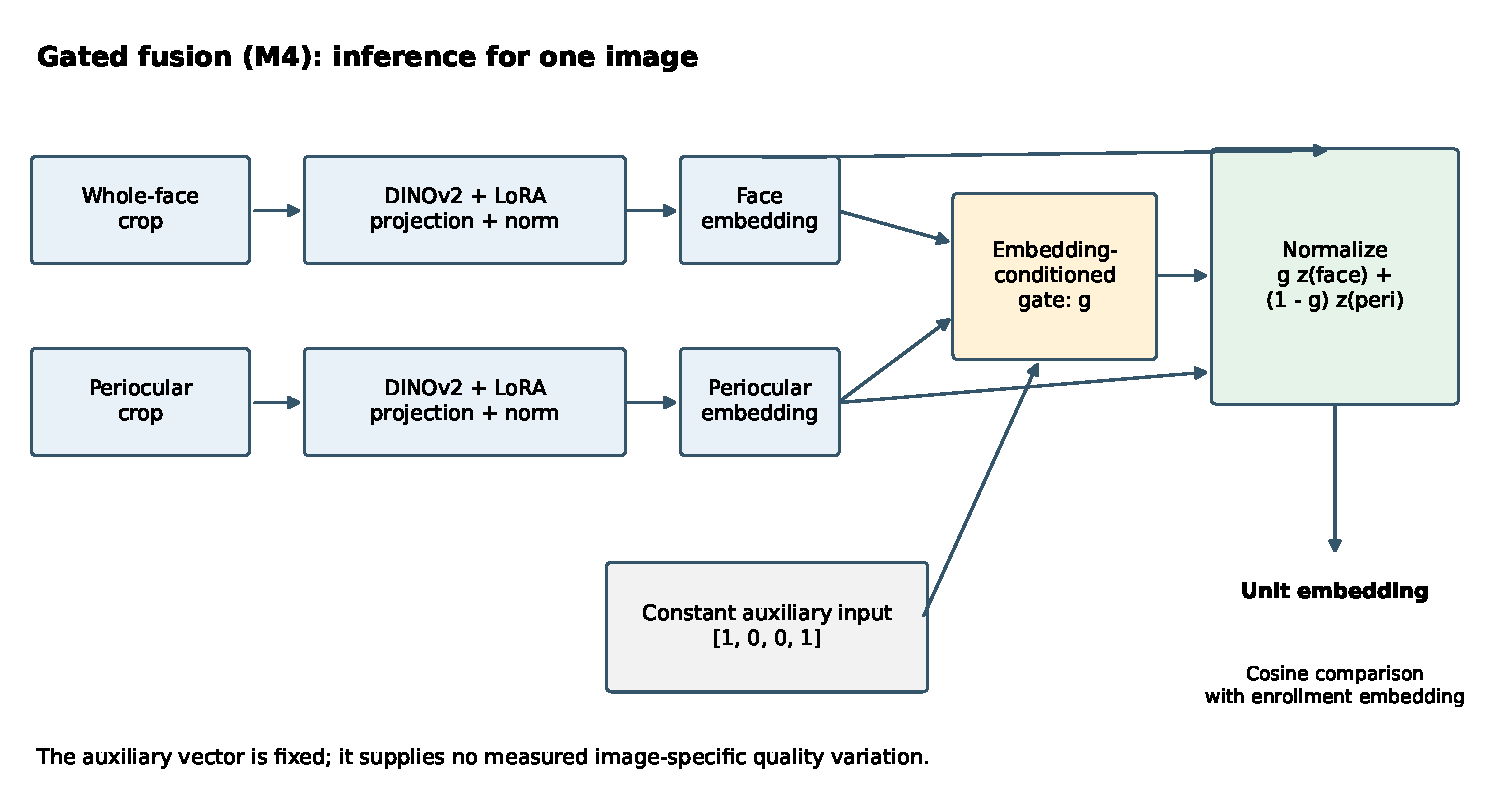
\includegraphics[width=\textwidth]{./fig_gated_architecture.pdf}
\caption{Executed gated-fusion inference path for one image. Both crop embeddings feed the gate and the normalized mixture. The auxiliary vector is constant, and the training-only identity classifier is omitted from this inference diagram. The enrollment image is processed by the same model before cosine comparison.}
\label{fig:thesismethod}
\end{figure}

\section{Representation branches}
Let $x_f$ be a standardized whole-face crop and $x_p$ be a periocular crop containing both eyes, eyebrows, the upper nose, and local context. Let $E_f$ and $E_p$ denote DINOv2 encoders and let $P_f$ and $P_p$ denote trainable projection heads. The normalized branch embeddings are
\begin{equation}
 z_f=\operatorname{norm}(P_f(E_f(x_f))),\qquad z_p=\operatorname{norm}(P_p(E_p(x_p))).
\end{equation}
The whole-face and periocular branches use the same image resolution and corresponding image normalization. Landmark failures are recorded in the crop manifest and are not silently replaced by a whole-face image.

\section{Fixed and learned fusion}
The fixed-fusion baseline combines both branches with equal weight:
\begin{equation}
 z_{\mathrm{fixed}}=\operatorname{norm}(0.5z_f+0.5z_p).
\end{equation}
The learned-fusion model computes a scalar mixing weight
\begin{equation}
 g=\sigma\left(\operatorname{MLP}([z_f;z_p;q_f;q_p])\right),
\end{equation}
where $q_f$ and $q_p$ denote auxiliary descriptor slots. Their values are constant in this experiment, as discussed below. The final embedding is
\begin{equation}
 z_{\mathrm{gate}}=\operatorname{norm}(gz_f+(1-g)z_p).
\end{equation}
The gate is treated as a learned fusion mechanism rather than a calibrated reliability estimator. Its input contains both branch embeddings and four auxiliary descriptors, but all new training and evaluation use the constant vector $[1,0,0,1]$. Historical auxiliary-input and cache-key defects are recorded separately and do not supply the new headline results. Consequently, this paper does not interpret the scalar gate value as a calibrated quality score. With constant auxiliary input, its first-layer contribution is a fixed bias. Any image-dependent change in the gate must therefore arise from the branch embeddings. We examine that dependence through gate distributions and controls that replace the learned weights.

\section{LoRA adaptation and training objective}
LoRA updates are inserted into the selected attention projection layers. The encoder's original parameters remain frozen, while LoRA parameters and projection/fusion heads are optimized. Let $h_i$ be the embedding for a training image and $y_i$ its training identity. The primary training objective is identity cross-entropy over the training identities:
\begin{equation}
 \mathcal{L}_{\mathrm{ID}}=-\sum_i\log p(y_i\mid h_i).
\end{equation}
Only training identities define classifier classes. EER and ROC-constrained TAR are retrospective summaries. Separately, validation identities determine thresholds that are frozen before test evaluation; both actual test FAR and TAR are reported at those thresholds. The verification score for two normalized embeddings is
\begin{equation}
 s(i,j)=z_i^\top z_j.
\end{equation}

\section{Ablation configurations}
Table~\ref{tab:ablations} separates the effects of adaptation, region selection, and fusion. M0 freezes the encoder but trains its projection; it is not an entirely untrained system.
\begin{table}[t]
\centering
\caption{Model configurations and the comparison each supports.}
\label{tab:ablations}
\begin{tabular}{cll}
\toprule
ID & Configuration & Purpose\\
\midrule
M0 & Frozen encoder + projection & Head baseline\\
M1 & Whole-face DINOv2 + LoRA & Adaptation effect\\
M2 & Periocular DINOv2 + LoRA & Periocular-only effect\\
M3 & Dual LoRA + fixed fusion & Fusion without gating\\
M4 & Dual LoRA + learned gate & Learned fusion\\
\bottomrule
\end{tabular}
\end{table}


\chapter{Datasets and Protocol}
\section{ROF content and identity audit}
The local ROF reconstruction contains 7,751 indexed files, 399 condition-specific labels, 182 normalized names, and 6,491 distinct file hashes. It excludes a resource illustration previously indexed as an identity. Its image inventory differs from the maintainer's published counts. All 437 local annotation pickles match the checked official Git blob hashes, but an acquisition log establishing the image download history was not located. Annotation provenance therefore does not certify every downloaded image or semantic label.

Condition suffixes are normalized before identity partitioning. The historical complete-case manifest had 7,295 rows; an exact-content audit found four rows of one image across training and validation under different names. A perceptual screen subsequently found a near-identical photograph under different names across training and test despite different file hashes. The new manifest excludes exact repetitions, undecodable content, the cross-label conflict, and both copies of the confirmed cross-split near-duplicate photograph. It contains 6,171 rows: 4,405 training, 844 validation, and 922 test images, with 128, 26, and 28 normalized identity labels respectively. File-hash uniqueness and label partition disjointness are checked before training. The manifest hash is recorded in every new checkpoint; historical checkpoints are not resumed into this experiment.

The new ROF protocol uses one neutral enrollment image per eligible identity and condition-specific probes. Self-image comparisons are excluded. The masked test protocol contains 423 pairs (47 genuine, 376 impostor) over nine eligible identity labels; sunglasses contains 6,648 pairs (277 genuine, 6,371 impostor) over 24; neutral contains 15,960 pairs (570 genuine, 15,390 impostor) over 28. Every model uses the same ordered pairs. Validation protocols are constructed only from validation identities, with 300 masked, 5,148 sunglasses, and 14,404 neutral pairs. The masked validation protocol has 30 genuine and 270 impostor pairs over ten eligible identities. This small identity coverage limits extrapolation.

\section{External protocols after recorded exclusions}
The original complete-case MFR2 protocol has 820 pairs. A normalized exact-name match identified one ROF training name, Joe Biden, affecting 18 pairs. Removing those pairs before the new evaluation leaves 802 pairs: 406 genuine and 396 impostor. This removes the known overlap; aliases, unrecognized identities, and overlap with backbone pretraining remain unknown. No MFR2 image is used for new gradient updates or threshold selection.

The RMFRD source index has 91,849 entries. Its historical exploratory verification protocol contained 22,554 pairs. The exact-content audit identified 36 source/crop conflict groups across nominal identities, affecting 756 pairs. Their exclusion leaves 21,798 pairs: 1,038 genuine and 20,760 impostor. This is an exact-conflict-excluded exploratory protocol, rather than an independently certified semantic identity benchmark. Perceptual duplicates and mislabeled photographs can remain. The same constant auxiliary vector is used on ROF, MFR2, and RMFRD, so missing external quality metadata cannot be interpreted as measured quality.

\section{Metrics, calibration, and uncertainty}
We report ROC-AUC, EER, and empirical TAR subject to FAR at most $10^{-2}$ and $10^{-3}$. These ROC operating points use the test scores retrospectively and are not deployment thresholds. All metrics are recomputed from saved ten-decimal raw scores. The first nonzero masked test FAR is $1/376\approx0.00266$; the $10^{-3}$ summary therefore uses the zero-observed-false-accept portion of this finite ROC. It does not demonstrate population FAR below $10^{-3}$.

For a separate calibration analysis, validation impostor scores set the most permissive threshold permitting at most $\lfloor\alpha N_{\rm val}^{-}\rfloor$ false accepts, with ties excluded using the next representable larger threshold. The threshold is frozen for the matching ROF test condition. MFR2 and RMFRD receive the ROF masked-validation threshold without external calibration. We report actual test false accepts, genuine accepts, FAR, and TAR, rather than naming the validation target as an achieved test FAR. At a masked validation target of $10^{-3}$, only zero observed validation false accepts are permitted because $N_{\rm val}^{-}=270$.

Seed variation is described by the arithmetic mean and sample standard deviation of three independently trained seeds, 7, 42, and 123. A distinct sensitivity analysis draws 1,000 multinomial identity-node bootstrap replicates, with RNG seed 42. If identity $i$ is drawn $c_i$ times, a same-identity edge receives weight $c_i$, and an impostor edge between $i$ and $j$ receives weight $c_i c_j$. This accounts for reuse of identities at both endpoints. The paired comparison applies the same weights to both systems and all three fixed training seeds, then averages their AUC differences within each replicate. The percentile interval is conditional on the trained checkpoints and selected identities; it does not quantify uncertainty over all possible training sets or establish a population security guarantee. Ten descriptive contrasts are reported without a multiple-comparison significance claim.

\chapter{Experimental Settings}
\textbf{Inputs and backbone.} Face and periocular crops are resized to $224\times224$ and normalized with ImageNet channel statistics. Both branches use DINOv2 ViT-B/14 with a 768-dimensional projected embedding. LoRA rank is 8, scaling is 16, and dropout is 0.1; query, key, and value attention projections receive the updates. Base encoder weights remain frozen.

\textbf{Optimization.} All 15 new models use CPU, eight PyTorch threads, five complete epochs, batch size 16, AdamW with learning rate $10^{-4}$ and weight decay $10^{-4}$, and identity cross-entropy over the 128 training labels. Each epoch draws 4,405 training samples uniformly with replacement, producing 276 batches, and each full run executes 1,380 optimizer steps. There is no smoke-test batch cap in a research run. Training-time classifiers do not contribute to verification scores. Final fifth-epoch checkpoints are evaluated without selecting a best epoch on test performance.

\textbf{Execution and recovery.} The executed environment records PyTorch 2.14.0+cpu, deterministic algorithms, and an offline cached DINOv2 model. Atomic checkpoints retain optimizer state, sample order, next batch, epoch losses, and Python, NumPy, and PyTorch RNG states. Manifest and source signatures reject incompatible resumes. The serial coordinator verifies completed score hashes before retaining a run. Periocular-only training skips the unused whole-face forward pass; this changes random-number consumption relative to the historical trainer, so the new experiment is not claimed to reproduce historical optimization bit for bit.

\section{Parameter efficiency}

\begin{table}[h]
\centering
\caption{Nominal parameter accounting at model construction; excludes the training-only classifier.}
\label{tab:params}
\begin{tabular}{lrrr}
\toprule
ID & Total parameters & Trainable & Trainable \%\\
\midrule
M0 & 87\,171\,072 & 590\,592 & 0.68\\
M1 & 87\,613\,440 & 1\,032\,960 & 1.18\\
M2 & 175\,226\,880 & 2\,065\,920 & 1.18\\
M3 & 175\,226\,880 & 2\,065\,920 & 1.18\\
M4 & 175\,424\,257 & 2\,263\,297 & 1.29\\
\bottomrule
\end{tabular}
\end{table}

Table~\ref{tab:params} reports nominal instantiated parameters. M0 trains a 590,592-parameter projection despite freezing the encoder. M2 instantiates an unused whole-face branch: only 1,032,960 parameters affect its returned periocular embedding, versus 2,065,920 nominal trainables. The training-only 128-class head adds 98,432 parameters and is excluded from this table. Every adapted variant therefore trains at most 2.26~M parameters (1.29\%) of a 175~M-parameter dual-encoder system. Hardware, available runtimes, software versions, and checkpoint hashes are recorded in the artifact. Peak memory was not instrumented.


\chapter{Results}
All results in this section come from the 15 newly trained models on the duplicate-excluded manifest. Historical numerical files are retained for audit and are not pooled with these runs. Tables distinguish the new protocol from earlier complete-case and post-hoc score-filtered analyses.

\section{Masked ROF verification}
Periocular LoRA has the highest masked mean AUC, 0.9221, followed by fixed fusion at 0.9134 and gating at 0.8989. Whole-face LoRA improves from the frozen projection baseline's 0.8303 to 0.8852. Thus adaptation improves ranking, and restricting attention to the upper face is useful under lower-face occlusion. The gated model does not recover the best periocular-only ranking. The gate-minus-fixed mean AUC difference is $-0.0145$, with a two-endpoint identity-resampling sensitivity interval of $[-0.0560,0.0144]$. Only nine masked test identities are eligible, so the interval is broad and the protocol supports a conditional comparison.

The low-FAR columns must be read with the finite denominator. A zero-observed-false-accept point can have nonzero TAR, but does not validate a security operating point below the first nonzero FAR step. The seed-42 ROC plot omits FAR-zero points on the logarithmic axis; those points remain included in metric computation.
\begin{table}[t]
\centering
\setlength{\tabcolsep}{2.2pt}
\caption{New ROF masked test: 47 genuine and 376 impostor pairs. Values are mean with sample seed SD in subscripts; three seeds. TAR columns are retrospective ROC summaries, not validation-calibrated test rates.}
\label{tab:rofmasked}
\begin{tabular}{lrrrr}
\toprule
Configuration & AUC & EER & TAR$_{.01}$ & TAR$_{.001}$\\
\midrule
Frozen + projection & .8303$_{\pm.024}$ & .2580$_{\pm.035}$ & .1348$_{\pm.033}$ & .0000$_{\pm.000}$\\
Whole LoRA & .8852$_{\pm.005}$ & .1711$_{\pm.004}$ & .2553$_{\pm.043}$ & .0780$_{\pm.012}$\\
Periocular LoRA & \textbf{.9221}$_{\pm.005}$ & \textbf{.1339}$_{\pm.009}$ & .0851$_{\pm.056}$ & .0142$_{\pm.012}$\\
Fixed fusion & .9134$_{\pm.007}$ & .1507$_{\pm.019}$ & .2908$_{\pm.033}$ & .1418$_{\pm.044}$\\
Learned gating & .8989$_{\pm.002}$ & .1711$_{\pm.020}$ & \textbf{.3191}$_{\pm.056}$ & \textbf{.1560}$_{\pm.054}$\\
\bottomrule
\end{tabular}
\end{table}
\begin{figure}[t]
\centering
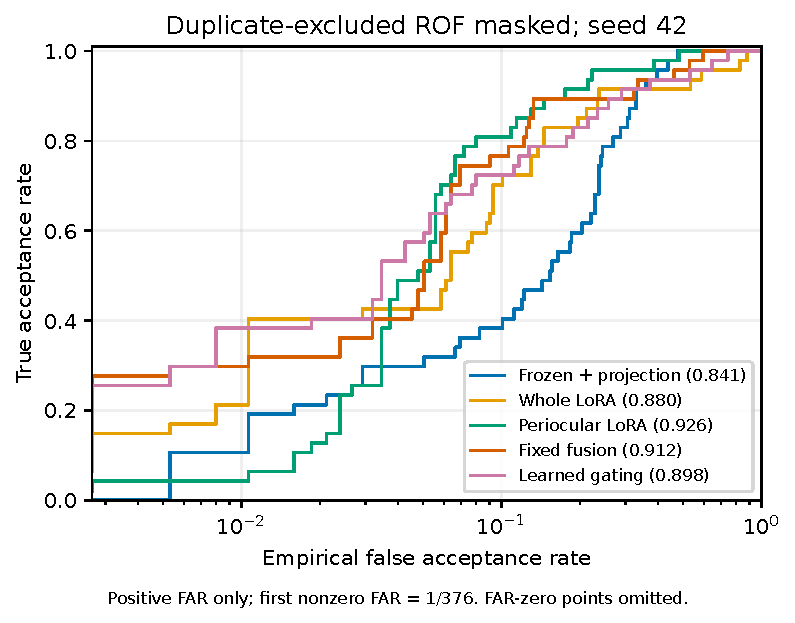
\includegraphics[width=\columnwidth]{fig_rof_masked_roc.pdf}
\caption{New masked ROF ROC, seed 42. Positive empirical FAR points only; first nonzero FAR is $1/376$. FAR-zero points are omitted from this logarithmic plot.}
\label{fig:rofmaskedroc}
\end{figure}

\section{Sunglasses and neutral ROF verification}
Sunglasses occlude the region used by the periocular-only model. Its mean AUC falls to 0.7905, below the frozen whole-face baseline at 0.8780. Fixed fusion leads at 0.8950, narrowly ahead of gating at 0.8924 and whole-face LoRA at 0.8913. The gated-minus-fixed difference is $-0.0026$, with sensitivity interval $[-0.0099,0.0061]$. These results show that the availability of a second branch does not ensure a gain from learned weighting.

On neutral images, learned gating has the largest mean AUC, 0.9458, compared with fixed fusion at 0.9428 and whole-face LoRA at 0.9413. The gated-minus-fixed difference is 0.0030, with sensitivity interval $[-0.0046,0.0106]$. This small ordering should not be interpreted as a conclusive population advantage. Periocular-only AUC is 0.8875, indicating information loss when clean lower-face cues are discarded. Table~\ref{tab:rofneutral} includes this neutral control so that cross-condition claims do not rely only on occluded probes.
\begin{table}[t]
\centering
\setlength{\tabcolsep}{2.2pt}
\caption{New ROF sunglasses test: 277 genuine and 6,371 impostor pairs. Values are mean with sample seed SD in subscripts; three seeds. TAR columns are retrospective ROC summaries, not validation-calibrated test rates.}
\label{tab:rofsunglasses}
\begin{tabular}{lrrrr}
\toprule
Configuration & AUC & EER & TAR$_{.01}$ & TAR$_{.001}$\\
\midrule
Frozen + projection & .8780$_{\pm.003}$ & .1774$_{\pm.004}$ & .1095$_{\pm.002}$ & .0132$_{\pm.004}$\\
Whole LoRA & .8913$_{\pm.002}$ & .1596$_{\pm.005}$ & \textbf{.1661}$_{\pm.010}$ & .0337$_{\pm.004}$\\
Periocular LoRA & .7905$_{\pm.014}$ & .2632$_{\pm.007}$ & .0710$_{\pm.010}$ & .0048$_{\pm.004}$\\
Fixed fusion & \textbf{.8950}$_{\pm.002}$ & \textbf{.1531}$_{\pm.008}$ & .1564$_{\pm.012}$ & .0144$_{\pm.006}$\\
Learned gating & .8924$_{\pm.006}$ & .1544$_{\pm.001}$ & .1384$_{\pm.016}$ & \textbf{.0373}$_{\pm.008}$\\
\bottomrule
\end{tabular}
\end{table}
\begin{table}[t]
\centering
\setlength{\tabcolsep}{2.2pt}
\caption{New ROF neutral test: 570 genuine and 15,390 impostor pairs. Values are mean with sample seed SD in subscripts; three seeds. TAR columns are retrospective ROC summaries, not validation-calibrated test rates.}
\label{tab:rofneutral}
\begin{tabular}{lrrrr}
\toprule
Configuration & AUC & EER & TAR$_{.01}$ & TAR$_{.001}$\\
\midrule
Frozen + projection & .9328$_{\pm.001}$ & .1503$_{\pm.001}$ & .2240$_{\pm.006}$ & \textbf{.0468}$_{\pm.006}$\\
Whole LoRA & .9413$_{\pm.002}$ & .1237$_{\pm.003}$ & \textbf{.2269}$_{\pm.063}$ & .0193$_{\pm.005}$\\
Periocular LoRA & .8875$_{\pm.005}$ & .1707$_{\pm.003}$ & .0942$_{\pm.006}$ & .0263$_{\pm.008}$\\
Fixed fusion & .9428$_{\pm.001}$ & .1146$_{\pm.002}$ & .1883$_{\pm.022}$ & .0310$_{\pm.017}$\\
Learned gating & \textbf{.9458}$_{\pm.003}$ & \textbf{.1122}$_{\pm.007}$ & .1965$_{\pm.024}$ & .0205$_{\pm.005}$\\
\bottomrule
\end{tabular}
\end{table}
\begin{figure}[t]
\centering
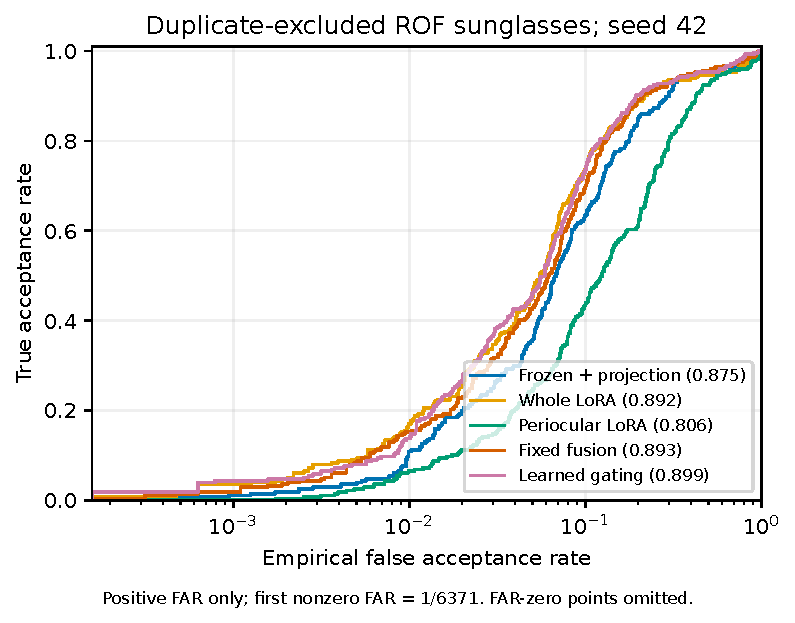
\includegraphics[width=\columnwidth]{fig_rof_sunglasses_roc.pdf}
\caption{New sunglasses ROF ROC, seed 42. Only positive empirical FAR points are plotted; all systems use the same frozen pairs.}
\label{fig:rofsunglassesroc}
\end{figure}

\section{Known-overlap-excluded MFR2}
Learned gating has the highest mean AUC on the 802 retained MFR2 pairs, 0.9548, compared with fixed fusion at 0.9398. The gated-minus-fixed difference is 0.0150, with identity-resampling interval $[0.0044,0.0283]$. Whole-face LoRA reaches 0.9360, compared with 0.8412 for the frozen baseline; the adaptation gain is larger than the gate-versus-fixed difference. No target-domain labels are used for gradient updates or calibration.

The known overlapping training name has been excluded, so these are not the earlier contaminated 820-pair headline results. However, exclusion by normalized exact name is not a complete identity audit. Unknown aliases and DINOv2 pretraining overlap remain possible. The external ROC describes ranking on the retained protocol; transferred ROF validation thresholds are evaluated separately.
\begin{table}[t]
\centering
\setlength{\tabcolsep}{2.2pt}
\caption{Known-name-overlap-excluded MFR2: 406 genuine and 396 impostor pairs. Values are mean with sample seed SD in subscripts; three seeds. TAR columns are retrospective ROC summaries, not validation-calibrated test rates.}
\label{tab:mfr2}
\begin{tabular}{lrrrr}
\toprule
Configuration & AUC & EER & TAR$_{.01}$ & TAR$_{.001}$\\
\midrule
Frozen + projection & .8412$_{\pm.006}$ & .2496$_{\pm.008}$ & .1453$_{\pm.013}$ & .0041$_{\pm.003}$\\
Whole LoRA & .9360$_{\pm.015}$ & .1406$_{\pm.018}$ & .2906$_{\pm.051}$ & .0476$_{\pm.051}$\\
Periocular LoRA & .9068$_{\pm.010}$ & .1647$_{\pm.017}$ & .2299$_{\pm.044}$ & .1355$_{\pm.020}$\\
Fixed fusion & .9398$_{\pm.005}$ & .1445$_{\pm.016}$ & \textbf{.3415}$_{\pm.067}$ & \textbf{.1741}$_{\pm.016}$\\
Learned gating & \textbf{.9548}$_{\pm.002}$ & \textbf{.1145}$_{\pm.005}$ & .2808$_{\pm.089}$ & .0172$_{\pm.010}$\\
\bottomrule
\end{tabular}
\end{table}
\begin{figure}[t]
\centering
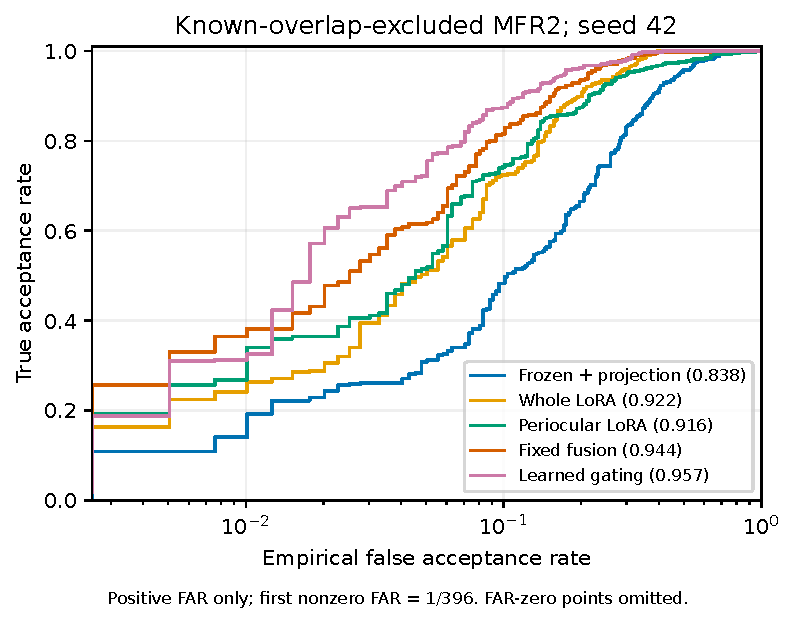
\includegraphics[width=\columnwidth]{fig_mfr2_roc.pdf}
\caption{MFR2 ROC after known training-name-overlap exclusion, seed 42; positive empirical FAR points only. Auxiliary inputs match training.}
\label{fig:mfr2roc}
\end{figure}

\section{Exact-conflict-excluded RMFRD}
Fixed fusion has the highest exploratory RMFRD mean AUC, 0.7240, followed by learned gating at 0.7175 and periocular LoRA at 0.7132. Whole-face LoRA reaches 0.7045 and the frozen baseline 0.6957. The gated-minus-fixed difference is $-0.0066$, with sensitivity interval $[-0.0135,0.0004]$. The completed descriptive interval includes zero; it neither establishes a conclusive ordering nor validates the dataset labels.

The much lower AUC than on MFR2 shows substantial transfer difficulty. Removing known exact conflicts avoids their direct influence, while remaining annotation and acquisition uncertainty prevents a strong unseen-identity or deployment claim. Figure~\ref{fig:crossauc} summarizes all five test conditions with seed variation rather than selecting one favorable dataset.
\begin{table}[t]
\centering
\setlength{\tabcolsep}{2.2pt}
\caption{Exact-conflict-excluded exploratory RMFRD: 1,038 genuine and 20,760 impostor pairs. Values are mean with sample seed SD in subscripts; three seeds. TAR columns are retrospective ROC summaries, not validation-calibrated test rates.}
\label{tab:rmfrd}
\begin{tabular}{lrrrr}
\toprule
Configuration & AUC & EER & TAR$_{.01}$ & TAR$_{.001}$\\
\midrule
Frozen + projection & .6957$_{\pm.004}$ & .3518$_{\pm.002}$ & .0267$_{\pm.004}$ & .0035$_{\pm.001}$\\
Whole LoRA & .7045$_{\pm.010}$ & .3507$_{\pm.011}$ & .0324$_{\pm.009}$ & .0045$_{\pm.001}$\\
Periocular LoRA & .7132$_{\pm.004}$ & .3412$_{\pm.005}$ & .0373$_{\pm.001}$ & .0035$_{\pm.002}$\\
Fixed fusion & \textbf{.7240}$_{\pm.010}$ & .3358$_{\pm.008}$ & \textbf{.0459}$_{\pm.003}$ & .0071$_{\pm.002}$\\
Learned gating & .7175$_{\pm.012}$ & \textbf{.3356}$_{\pm.010}$ & .0421$_{\pm.004}$ & \textbf{.0083}$_{\pm.002}$\\
\bottomrule
\end{tabular}
\end{table}
\begin{figure}[t]
\centering
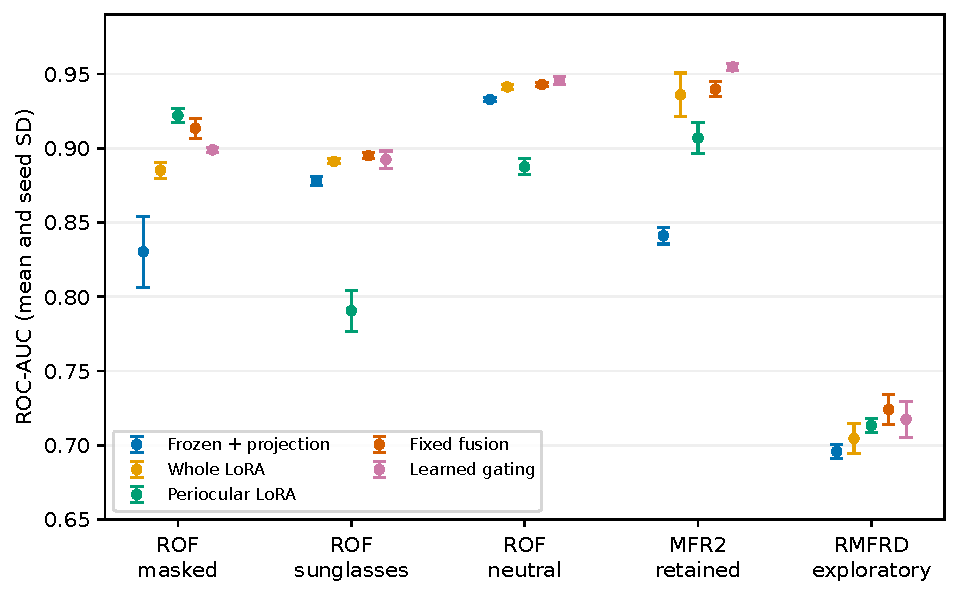
\includegraphics[width=\columnwidth]{fig_auc_cross_dataset.pdf}
\caption{New CPU-trained models: mean AUC and one sample SD across three seeds. MFR2 excludes the known overlapping name; RMFRD excludes known exact-content conflicts and remains exploratory.}
\label{fig:crossauc}
\end{figure}

\section{Validation-calibrated operating points}
Table~\ref{tab:calibration} reports the gated system at a validation target FAR of 0.01. Each entry shows mean test TAR and FAR; acceptance counts are listed in seed order 7/42/123. ROF uses its matching validation condition, while both external datasets use ROF masked validation. The observed test FAR can exceed the validation target. In particular, the neutral test distribution produces appreciably more false accepts than the validation calibration suggests. This discrepancy is obscured if retrospective test ROC points are presented as preselected thresholds.

At validation target 0.001, masked calibration allows zero observed validation false accepts. That finite-sample event does not certify a population FAR of 0.001. Full per-seed thresholds, calibration and test counts, and both targets are included for all models in the machine-readable reports. Calibration is fixed by the stated rule and is not revised after observing test errors.
\begin{table}[t]
\centering
\caption{Gated model at validation target FAR 0.01. Means over three seeds; TA/FA list actual test accept counts in seed order. External thresholds are transferred from masked ROF validation.}
\label{tab:calibration}
\begin{tabular}{lrrrr}
\toprule
Protocol & TAR & FAR & TA & FA\\
\midrule
Masked & 0.3546 & 0.0222 & 16/18/16 & 13/5/7\\
Sunglasses & 0.1252 & 0.0089 & 37/27/40 & 74/46/50\\
Neutral & 0.5076 & 0.0325 & 278/285/305 & 491/424/585\\
MFR2 & 0.6814 & 0.0396 & 299/264/267 & 21/10/16\\
RMFRD & 0.6426 & 0.3230 & 765/569/667 & 8417/5424/6273\\
\bottomrule
\end{tabular}
\end{table}

\section{Same-branch gate controls}
Training separate fixed and gated models changes both their branch features and their fusion rule. To isolate the latter, each trained gated checkpoint is also evaluated with its own branches under constant 0.5, validation-mean, and permuted weights, plus the individual branches. A validation-mean weight is calculated only from validation endpoints. Permutation uses seed 42 within unique endpoints of each protocol, with no cross-protocol mixing. It is a post-hoc diagnostic, not a deployable fusion policy or a new training run.

\begin{table}[t]
\centering
\caption{Mean AUC of fusion controls on the same trained gated branches. These are distinct from separately trained M3.}
\label{tab:gatecontrols}
\begin{tabular}{lrrrr}
\toprule
Protocol & Learned & Equal & Val. mean & Permuted\\
\midrule
Masked & 0.8989 & 0.9250 & 0.8946 & 0.8992\\
Sunglasses & 0.8924 & 0.8854 & 0.8934 & 0.8942\\
Neutral & 0.9458 & 0.9421 & 0.9464 & 0.9428\\
MFR2 & 0.9548 & 0.9512 & 0.9420 & 0.9391\\
RMFRD & 0.7175 & 0.7126 & 0.7181 & 0.7162\\
\bottomrule
\end{tabular}
\end{table}

On masked ROF, equal weighting of the gated model's branches gives mean AUC 0.9250, above learned weighting at 0.8989. The validation-mean gate also slightly exceeds learned gating on sunglasses and neutral images. Permuting weights gives 0.8942 on sunglasses, compared with learned weighting at 0.8924. MFR2 is more favorable to image-dependent gating: learned weighting gives 0.9548 versus 0.9420 with the validation-mean weight and 0.9391 after permutation. Thus evidence for useful sample-dependent weighting is protocol-specific rather than universal.

Mean gate values across seeds range from 0.709 to 0.749 on masked ROF and from 0.825 to 0.841 on sunglasses, assigning more weight to the face branch under sunglasses. Within-seed variation remains nonzero. This pattern is consistent with condition-dependent use of the branches, but does not establish calibrated reliability or causal detection of occlusion. Folding the constant auxiliary input into the first-layer bias changes gate outputs by at most $1.20\times10^{-7}$ across the recorded checks. The auxiliary fields therefore supply no measured image-specific quality information.
\begin{figure}[t]
\centering
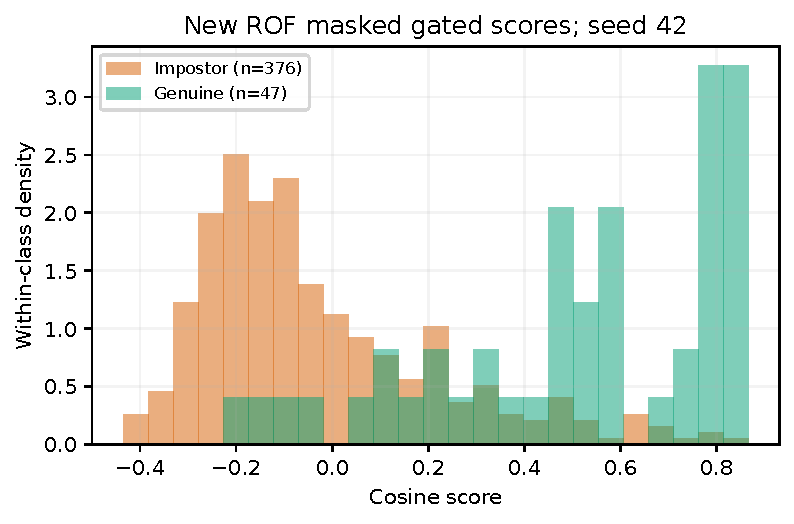
\includegraphics[width=\columnwidth]{fig_rof_masked_scores.pdf}
\caption{New masked ROF gated-fusion scores, seed 42. Shared bins; each class is normalized separately. Genuine and impostor counts remain visible.}
\label{fig:scores}
\end{figure}

\begin{table}[t]
\centering
\caption{Mean face-branch gate weight by protocol and training seed; within-endpoint SD in parentheses. These are descriptive gate outputs, not calibrated reliability probabilities.}
\label{tab:gatedistribution}
\begin{tabular}{lrrr}
\toprule
Protocol & Seed 7 & Seed 42 & Seed 123\\
\midrule
Masked & 0.712 (0.118) & 0.709 (0.100) & 0.749 (0.092)\\
Sunglasses & 0.841 (0.082) & 0.825 (0.083) & 0.830 (0.082)\\
Neutral & 0.773 (0.107) & 0.767 (0.096) & 0.778 (0.099)\\
MFR2 & 0.659 (0.118) & 0.632 (0.117) & 0.696 (0.103)\\
RMFRD & 0.745 (0.086) & 0.697 (0.090) & 0.775 (0.071)\\
\bottomrule
\end{tabular}
\end{table}
\section{Pretrained face-recognition diagnostic}
The artifact also evaluates OpenCV SFace \cite{sface} (December 2021 weights) using YuNet \cite{yunet} (March 2023) detection, five-landmark alignment, confidence threshold 0.8, and the detection closest to the image center. No target fine-tuning is performed. Failed pair detections receive score $-1$ and remain in the primary denominator; detected-only metrics are secondary. SFace reaches AUC 0.9399 on masked ROF, 0.9440 on sunglasses, 0.9991 on neutral, 0.9968 on retained MFR2, and 0.8187 on retained RMFRD. Respectively, 9, 48, 0, 0, and 1,155 pairs contain failed detections. The published ledger records the actual endpoints and raw scores.

These results exceed the mean AUC of the new DINOv2 variants on each listed protocol, but the comparison is not matched for pretraining data, identity exposure, detector, alignment, or training objective. It is a diagnostic showing that this ablation study does not establish state-of-the-art face verification. A matched modern face-recognition baseline and independent external labels would be required for a stronger comparative claim.

\begin{table}[t]
\centering
\caption{SFace diagnostic on the same retained test protocols. Failed pairs receive score $-1$ and remain in the denominator. Different pretraining and alignment prevent a matched architecture claim.}
\label{tab:sface}
\begin{tabular}{lrr}
\toprule
Protocol & AUC & Failed pairs\\
\midrule
Masked & 0.9399 & 9\\
Sunglasses & 0.9440 & 48\\
Neutral & 0.9991 & 0\\
MFR2 & 0.9968 & 0\\
RMFRD & 0.8187 & 1155\\
\bottomrule
\end{tabular}
\end{table}
\section{Paired comparison record}
Table~\ref{tab:paired} gives every prespecified descriptive contrast from the completed summary, including unfavorable directions. Positive differences favor the first model. The same resampled identity counts are applied to both models and all three training seeds; differences are averaged within each replicate. These intervals condition on the fitted checkpoints and frozen protocols. They are not confidence intervals for performance on an arbitrary future population.
\begin{table}[t]
\centering
\caption{Paired mean AUC differences and two-endpoint identity-resampling 95\% sensitivity intervals; 1,000 replicates. G--F denotes gated minus fixed fusion; W--B denotes whole LoRA minus frozen baseline.}
\label{tab:paired}
\begin{tabular}{llrrr}
\toprule
Protocol & Contrast & Difference & Lower & Upper\\
\midrule
Masked & G--F & -0.0145 & -0.0560 & 0.0144\\
Masked & W--B & 0.0549 & -0.0424 & 0.1697\\
Sunglasses & G--F & -0.0026 & -0.0099 & 0.0061\\
Sunglasses & W--B & 0.0133 & -0.0030 & 0.0366\\
Neutral & G--F & 0.0030 & -0.0046 & 0.0106\\
Neutral & W--B & 0.0085 & -0.0117 & 0.0274\\
MFR2 & G--F & 0.0150 & 0.0044 & 0.0283\\
MFR2 & W--B & 0.0948 & 0.0513 & 0.1474\\
RMFRD & G--F & -0.0066 & -0.0135 & 0.0004\\
RMFRD & W--B & 0.0088 & -0.0067 & 0.0263\\
\bottomrule
\end{tabular}
\end{table}
A positive or negative interval on an audited subset cannot resolve selection bias in that subset. Exclusion rules were fixed before these new runs, but they were motivated by defects found during the earlier experiment. The prospective retraining removes the direct influence of those known images; it does not turn the local reconstruction into a newly collected independent cohort. The provenance records identify the revised experiment so that its numbers cannot be mistaken for measurements from the original complete-case protocol.
\chapter{Discussion}
\section{Adaptation and regional complementarity}
Whole-face LoRA improves mean AUC over the frozen projection baseline on every test protocol, supporting the direction of H1. The gain is largest on MFR2 and masked ROF and smaller on RMFRD. This comparison establishes an effect of supervised adaptation within the present experiment. It does not show that adapting a general visual encoder is preferable to using a face-specific pretrained model.

The answer to RQ2 depends on which region remains visible. Periocular LoRA leads the masked comparison, but performs poorly under sunglasses and loses useful information on neutral faces. H2 is therefore supported in a limited sense: the upper face is an effective source of identity evidence under lower-face occlusion, but is not a sufficient representation for all three conditions. Fixed fusion is a strong baseline because it can retain information from both regions without learning a separate weighting policy.

The answer to RQ3 is less favorable to learned weighting. The gated model leads mean AUC on MFR2 and neutral ROF, but not on masks, sunglasses, or RMFRD. Several paired sensitivity intervals include zero. More importantly, the same-branch controls show that its inference rule is not consistently responsible for the quality of its representation. Equal weights improve masked AUC for the trained gated branches, and a constant validation-mean weight remains competitive on ROF. The evidence does not support treating a learned gate as an automatic improvement in robustness.

\section{AUC, calibration, and deployment}
AUC describes ranking over the full score range, whereas a deployed verifier uses a particular threshold. A small AUC gain can coexist with poor TAR at a strict FAR constraint. The saved validation-calibrated counts demonstrate distribution shift directly: a threshold satisfying a validation target does not necessarily attain that rate on new identities. This is especially important for neutral scores, where many reused enrollment and probe identities make nominal pair counts look larger than the amount of independent information.

The masked test protocol has only 47 genuine comparisons and nine eligible labels. One changed genuine accept shifts TAR by $1/47$, and one changed impostor accept shifts FAR by $1/376$. Reporting four decimal places aids arithmetic verification but does not imply four-decimal statistical precision. Identity-node resampling is a sensitivity analysis of this finite protocol, not a substitute for collecting more independent identities and sessions.

The score-distribution plot illustrates overlap between genuine and impostor scores without diagnosing the identity or cause of individual errors. Qualitative identity-label decisions require human review of licensed source data. The retained manifests and exclusion ledgers make such review possible without distributing private or restricted face images in the repository.

\section{Positioning and negative findings}
Face--periocular fusion, LoRA, and quality-dependent weighting all have established precedents. The scientific value of this experiment lies in testing their roles separately and reporting where the expected benefit fails. In particular, a favorable comparison between two jointly trained systems is not enough to attribute the difference to adaptive weighting. The same-branch controls provide a more direct diagnostic of that inference policy.

The SFace results set a further boundary on the contribution. They show that a face-specific pretrained model can obtain stronger ranking performance on these protocols, although different training data and alignment prevent a matched architecture comparison. The present study should therefore be read as an ablation and reproducibility study. Claims of competitive face recognition would require matched baselines, a broader identity sample, and independent label checks.

\enlargethispage{\baselineskip}
The constant auxiliary vector also changes how the method should be described. The architecture accepts descriptor inputs, but this experiment supplies no varying quality measurement. The gate can react to its embeddings; it cannot demonstrate the value of measured quality cues. A future quality-aware study would need validated descriptors and controlled descriptor ablations, with its evaluation rule fixed before the test results are inspected.

\chapter{Limitations and Threats to Validity}
The duplicate-excluded manifest removes the known exact conflicts and confirmed cross-split near-duplicate photograph; it does not certify all semantic labels or exhaustively detect perceptual duplicates. The annotation-source match does not resolve the local image acquisition discrepancy. Exact normalized-name overlap checks can miss aliases. Public-figure images may also appear in DINOv2 or SFace pretraining; those identity exposures are unknown.

Only three training initializations are measured. Seed SD is descriptive, and the node-bootstrap intervals condition on those three fitted systems and the frozen identity graph. Identity resampling cannot recreate missing acquisition sessions or repair mislabeled photographs. The ten contrasts are exploratory without family-wise error control. The small masked identity set and finite impostor denominator preclude strong security claims at very low FAR.

RMFRD remains exploratory after exact-conflict exclusion. MFR2's retained protocol removes one known overlap rather than proving all identities unseen. SFace uses different alignment and pretraining, preventing a controlled architecture ranking. Peak memory was not instrumented. Logged wall-clock training durations include interruptions or sleep and should not be treated as uninterrupted throughput benchmarks. CPU determinism was configured and checkpoint recovery tested within the recorded runtime, but bitwise reproduction across package versions or hardware is not asserted.

\chapter{Reproducibility and Artifact Specification}
The release contains the completed 15-model grid, 120 ordered raw-score files covering eight validation/test/external protocols, per-run evaluation reports, final training-progress records, checkpoint hashes, and the 25-row five-condition metric summary. Ten paired three-seed AUC comparisons include per-seed deltas, bootstrap configuration, and conditional intervals. The exact executed trainer, evaluator, common utilities, and model/metric runtime snapshots are shipped with source hashes; changing those sources invalidates the recorded execution signatures.

The reproducibility sequence is to obtain licensed images, restore the documented face/periocular paths, verify the frozen training and pair manifests, prepare the recorded software environment and DINOv2 cache, and run the CPU coordinator. Each model is trained for five epochs, scored on the same eight protocols, and summarized only after complete evaluation. A file lock prevents duplicate coordinators. Repeated launches retain verified completed runs; interruptions resume from atomic optimizer and RNG checkpoints rather than restarting the experiment. The repository does not include the face images, pretrained weight binaries, or approximately 10~GB of new trained checkpoints. Their recorded hashes permit local provenance checks but do not replace access to the binaries for inference reproduction.

Arithmetic verification can be performed without torch, images, or checkpoints: the release verifier independently reconstructs ROC metrics from raw scores, checks frozen-pair alignment and hashes, recalculates seed means and SDs, and checks manuscript table values. It separately retains the 90 historical metric files, historical sensitivities, and corrected historical MFR2 inference. Passing these checks means that the recorded files are internally consistent; it does not certify scientific novelty, journal acceptance, or semantic image labels.

Historical manuscript and interim follow-up snapshots remain under the history directory. Their claims and numerical tables are superseded by the completed CPU experiment in the current paper. No historical score filtering is represented as new training, and no incomplete or smoke-limited run supplies a headline table. Shared IEEE and arXiv substantive text and vector figures are regenerated together from the completed result evidence.

\chapter{Conclusion}
This study compared five parameter-efficient whole-face and periocular configurations using fifteen newly trained CPU models. No configuration led every condition. Periocular LoRA achieved the highest masked mean AUC (0.9221), fixed fusion led sunglasses (0.8950) and exploratory RMFRD (0.7240), and learned fusion led neutral ROF (0.9458) and retained MFR2 (0.9548).

The controls explain why those rankings need careful interpretation. A learned model can acquire useful branch representations without learning the best weights for combining them. Constant weighting can remain competitive, and validation-calibrated thresholds can produce a different test FAR from the intended target. Regional complementarity is supported by the evidence; universal adaptive robustness and deployment security are not.

The released scores, frozen protocols, and execution records make the reported experiment auditable. Broader independent identities, matched face-specific baselines, semantic label review, and a resolved ethics and permissions statement remain necessary for stronger claims and submission clearance.



\appendix
\chapter{Mathematical Foundations}
\section{Verification as a decision problem}
A verifier receives two images and produces a score. In this experiment the score is a cosine similarity between normalized embeddings. If $z_i$ and $z_j$ have unit Euclidean norm, then
\begin{equation}
s(i,j)=z_i^{\top}z_j.
\end{equation}
The score orders the evidence but does not itself decide whether to accept a claimed identity. A threshold $\tau$ gives the rule $s(i,j)\geq\tau$. Increasing the threshold usually rejects more impostor comparisons and more genuine comparisons. This trade-off is the reason a ranking metric and an operating-point metric answer different questions.

For genuine scores $\mathcal G$ and impostor scores $\mathcal I$, the empirical rates are
\begin{align}
\TAR(\tau)&=\frac{1}{|\mathcal G|}\sum_{s\in\mathcal G}\mathbf 1[s\geq\tau],\\
\FAR(\tau)&=\frac{1}{|\mathcal I|}\sum_{s\in\mathcal I}\mathbf 1[s\geq\tau].
\end{align}
The denominators are as important as the decimal rates. In the masked test protocol, one changed impostor acceptance changes FAR by $1/376$, while one changed genuine acceptance changes TAR by $1/47$. Reporting a small nominal FAR cannot overcome this finite resolution.

The ROC curve evaluates the decision at every score boundary. Its AUC can also be understood as the fraction of genuine--impostor score orderings that are correct, assigning half credit to ties. EER summarizes the crossing of false-accept and false-reject rates. Neither statistic chooses a deployment threshold independently of the test data.

\section{What low-rank adaptation changes}
For a frozen weight matrix $W_0\in\mathbb R^{d_{\rm out}\times d_{\rm in}}$, a LoRA update has the form
\begin{equation}
W=W_0+\frac{\alpha}{r}BA,
\qquad A\in\mathbb R^{r\times d_{\rm in}},\quad
B\in\mathbb R^{d_{\rm out}\times r}.
\end{equation}
The factorization introduces $r(d_{\rm in}+d_{\rm out})$ parameters for that update, instead of optimizing every entry of $W_0$. The experiment uses rank $r=8$ and scaling parameter $\alpha=16$ on attention query, key, and value projections. Projection heads and, where present, the fusion network also receive gradients.

Parameter efficiency concerns the optimized weights. The base transformer still performs its forward computation, and a two-encoder system still evaluates two image branches. A small trainable fraction is therefore not evidence of an equivalent reduction in inference time, peak memory, or energy. Those quantities require their own measurements. The nominal parameter table also includes an unused instantiated whole-face branch for the periocular-only configuration; the executed forward pass skips that branch.

\section{Why gate controls are necessary}
The training objective sends gradients through the fusion rule into both branches. Changing from fixed to learned fusion can therefore change the representation itself. Comparing two independently trained models combines these effects. It cannot, on its own, attribute the observed difference to the gate used at inference.

The same-branch controls hold the trained embeddings fixed and change only their combination. Equal weighting tests whether adaptive weights are needed at all. The validation-mean gate supplies a constant learned from validation endpoints. Permutation tests whether attaching a particular gate value to a particular image matters within the selected protocol. Individual-branch controls show what the jointly trained face and periocular representations can do separately. These are diagnostic comparisons of a trained system, not substitutes for a randomized study of all possible training procedures.

The auxiliary input is constant. A constant term in the first affine layer can be absorbed into its bias, which explains the numerical folding check. Variation in gate outputs must come from the embeddings rather than measured quality variation. A value such as $g=0.8$ consequently means a mixing coefficient; it is not an 80\% probability that the face is reliable.

\section{Calibration and dependent comparisons}
Validation calibration fixes $\tau$ using impostor comparisons from validation identities. When scores tie at the acceptance boundary, the rule excludes the boundary tie group rather than allowing more false accepts than the specified integer budget. Test scores are then evaluated at that frozen threshold. A shift in the score distribution can change test FAR even if the validation budget was satisfied exactly.

Pairs are not independent observations when one identity occurs in many comparisons. The node-resampling sensitivity analysis draws identities and weights their associated edges. Genuine edges receive the sampled multiplicity of their shared identity; impostor edges receive the product of the two endpoint multiplicities. Using the same weights for two models preserves their pairing. The result describes sensitivity to the observed identity graph and the three fitted seeds. It does not remove label error or uncertainty about an unobserved population.

\chapter{Experiment Register and Evidence Map}
\section{Completed experiment}
The completed grid contains five variants, each trained with seeds 7, 42, and 123. Every full run has five epochs and 1,380 optimizer steps. Validation is used for the specified threshold and gate-mean rules, while the final fifth-epoch model is used for evaluation. No model is selected by its test AUC. Smoke runs are isolated from the research outputs.

\begin{table}[htbp]
\centering
\caption{Mean AUC and sample seed SD in the completed experiment.}
\label{tab:thesisregister}
\begin{tabular}{llrr}
\toprule
Protocol & Variant & Mean AUC & Seed SD\\
\midrule
ROF masked & Frozen + projection & 0.830315 & 0.024009\\
ROF masked & Whole LoRA & 0.885186 & 0.005234\\
ROF masked & Periocular LoRA & 0.922061 & 0.004552\\
ROF masked & Fixed fusion & 0.913441 & 0.006606\\
ROF masked & Learned fusion & 0.898936 & 0.001884\\
ROF sunglasses & Frozen + projection & 0.877989 & 0.003140\\
ROF sunglasses & Whole LoRA & 0.891257 & 0.001719\\
ROF sunglasses & Periocular LoRA & 0.790531 & 0.013856\\
ROF sunglasses & Fixed fusion & 0.894972 & 0.002127\\
ROF sunglasses & Learned fusion & 0.892374 & 0.005800\\
ROF neutral & Frozen + projection & 0.932790 & 0.001199\\
ROF neutral & Whole LoRA & 0.941304 & 0.001512\\
ROF neutral & Periocular LoRA & 0.887455 & 0.005384\\
ROF neutral & Fixed fusion & 0.942830 & 0.001371\\
ROF neutral & Learned fusion & 0.945826 & 0.002609\\
MFR2 retained & Frozen + projection & 0.841164 & 0.005662\\
MFR2 retained & Whole LoRA & 0.935973 & 0.014746\\
MFR2 retained & Periocular LoRA & 0.906825 & 0.010288\\
MFR2 retained & Fixed fusion & 0.939767 & 0.004923\\
MFR2 retained & Learned fusion & 0.954794 & 0.002203\\
RMFRD exploratory & Frozen + projection & 0.695724 & 0.004475\\
RMFRD exploratory & Whole LoRA & 0.704538 & 0.010296\\
RMFRD exploratory & Periocular LoRA & 0.713228 & 0.004494\\
RMFRD exploratory & Fixed fusion & 0.724015 & 0.009870\\
RMFRD exploratory & Learned fusion & 0.717452 & 0.012143\\
\bottomrule
\end{tabular}
\end{table}

\section{Connecting questions to evidence}
RQ1 is answered by the whole-face LoRA and frozen-projection comparison. Both use a face input; the relevant change is encoder adaptation. RQ2 uses the periocular-only model and its contrast with whole-face and fusion models across masks, sunglasses, and neutral faces. RQ3 uses both separately trained fixed/gated models and the same-branch inference controls. Calibration analysis adds the separate question of whether thresholds transfer from validation identities to the held-out protocol.

The tests are deliberately not collapsed into a single winning model. Selecting a method for masked ranking is different from selecting one for neutral ranking or threshold transfer. The report therefore includes unfavorable directions and the stronger unmatched SFace diagnostic. That comparison helps set the scope of the claim, while its different pretraining and alignment prevent a controlled architecture conclusion.

\section{Where each claim can be checked}
The artifact's results/cpu\_clean directory contains the fifteen evaluation reports, final training records, and 120 raw-score files. Each report records eight protocols, input hashes, checkpoint hashes, metrics, calibration counts, and gate controls where applicable. The summary contains 25 condition--variant rows and ten paired mean-AUC comparisons. The frozen training and ROF pair manifests are under manifests/cpu\_followup; the retained external pair lists are under manifests/cleaned.

The executed source snapshots are under reproduction/research\_completion\_2026-11-02. The standard-library verifier can reconstruct score-level metrics and calibrated counts without images or torch. Embedding regeneration needs the licensed image/crop inputs and model weights, which are not distributed in the artifact. Hashes identify binaries but do not reconstruct them.

\chapter{Dataset Provenance and Submission Status}
\section{Sources and execution copies}
The original source identifiers are the ROF repository at \url{https://github.com/ekremerakin/RealWorldOccludedFaces}, the MFR2 maintainer page at \url{https://sites.google.com/view/masktheface/mfr2-dataset}, and the RMFRD repository at \url{https://github.com/X-zhangyang/Real-World-Masked-Face-Dataset}. Project workflows identify a Kaggle package named sangiyaparara/tbiom-dataset. Captured MFR2 and RMFRD run paths identify a second package named sangiyaparara/research-dataset. These are execution-copy identifiers; their presence does not establish the original acquisition dates or permissions for every image.

The ROF annotation audit matches 437 local files to the recorded upstream tree. Its scope is limited to the annotations. The local image counts differ from the maintainer's inventory, and a complete image acquisition log was not found. The source-trace document preserves the supporting local excerpts and their file hashes.

\section{Author decisions that remain}
The author reports that the work has not been submitted elsewhere. No submission has been performed by the drafting agent. An ethics/consent explanation, applicable dataset permissions, correspondence details, and any earlier public thesis or preprint version still require confirmation. Downloading an existing dataset is evidence about acquisition, not a substitute for those declarations.

The scientific contribution also needs author assessment against the intended venue. The experiment is reproducible at score level and distinguishes useful regional information from successful adaptive weighting. It does not establish a state-of-the-art result. Stronger claims require matched modern baselines, broader independent identities, and semantic label review. These limitations should be resolved or explained, rather than removed to make the document sound more conclusive.

Institution-specific title pages, approval pages, supervisor details, degree wording, and formatting are deliberately not invented. This report can be adapted when the actual university template is provided. The journal manuscript remains a separate ten-page document, and the research result files are shared between the two presentations.

\chapter*{Acknowledgments}
OpenAI ChatGPT assisted with drafting and revising prose in the Abstract, Introduction, Related Work, Research Questions, Methods, Datasets and Protocol, Experimental Settings, Results, Discussion, Limitations, Conclusion, and reproducibility documentation, and with implementation and checking of evaluation, verification, protocol-cleaning, and figure-generation scripts. Numerical measurements are computed by the documented experimental code from image embeddings or archived scores; generated prose is not used as experimental data. The author is responsible for validating the revised code, measurements, and manuscript before submission.
\begin{thebibliography}{00}
\bibitem{dinov2} M. Oquab \textit{et al.}, ``DINOv2: Learning robust visual features without supervision,'' \textit{Transactions on Machine Learning Research}, 2024.
\bibitem{dino} M. Caron, H. Touvron, I. Misra, H. J\'egou, J. Mairal, P. Bojanowski, and A. Joulin, ``Emerging properties in self-supervised vision transformers,'' in \textit{Proc. ICCV}, 2021, pp. 9650--9660.
\bibitem{mae} K. He, X. Chen, S. Xie, Y. Li, P. Doll\'ar, and R. Girshick, ``Masked autoencoders are scalable vision learners,'' in \textit{Proc. CVPR}, 2022, pp. 16000--16009.
\bibitem{simclr} T. Chen, S. Kornblith, M. Norouzi, and G. Hinton, ``A simple framework for contrastive learning of visual representations,'' in \textit{Proc. ICML}, 2020, pp. 1597--1607.
\bibitem{clip} A. Radford, J. W. Kim, C. Hallacy, A. Ramesh, G. Goh, S. Agarwal, G. Sastry, A. Askell, P. Mishkin, J. Clark, G. Krueger, and I. Sutskever, ``Learning transferable visual models from natural language supervision,'' in \textit{Proc. ICML}, 2021, pp. 8748--8763.
\bibitem{lora} E. J. Hu, Y. Shen, P. Wallis, Z. Allen-Zhu, Y. Li, S. Wang, L. Wang, and W. Chen, ``LoRA: Low-rank adaptation of large language models,'' in \textit{Proc. ICLR}, 2022.
\bibitem{vpt} M. Jia, L. Tang, B.-C. Chen, C. Cardie, S. Belongie, B. Hariharan, and S.-N. Lim, ``Visual prompt tuning,'' in \textit{Proc. ECCV}, 2022, pp. 709--727.
\bibitem{prompt} B. Lester, R. Al-Rfou, and N. Constant, ``The power of scale for parameter-efficient prompt tuning,'' in \textit{Proc. EMNLP}, 2021, pp. 3045--3059.
\bibitem{sphereface} W. Liu, Y. Wen, Z. Yu, M. Li, B. Raj, and L. Song, ``SphereFace: Deep hypersphere embedding for face recognition,'' in \textit{Proc. IEEE CVPR}, 2017, pp. 212--220.
\bibitem{cosface} H. Wang, Y. Wang, Z. Zhou, X. Ji, D. Gong, J. Zhou, Z. Li, and W. Liu, ``CosFace: Large margin cosine loss for deep face recognition,'' in \textit{Proc. IEEE CVPR}, 2018, pp. 5265--5274.
\bibitem{arcface} J. Deng, J. Guo, N. Xue, and S. Zafeiriou, ``ArcFace: Additive angular margin loss for deep face recognition,'' in \textit{Proc. IEEE CVPR}, 2019, pp. 4690--4699.
\bibitem{magface} Q. Meng, S. Zhao, Z. Huang, and F. Zhou, ``MagFace: A universal representation for face recognition and quality assessment,'' in \textit{Proc. IEEE CVPR}, 2021, pp. 14225--14234.
\bibitem{adaface} M. Kim, A. K. Jain, and X. Liu, ``AdaFace: Quality adaptive margin for face recognition,'' in \textit{Proc. IEEE CVPR}, 2022, pp. 18750--18759.
\bibitem{rof} M. E. Erak{\i}n, U. Demir, and H. K. Ekenel, ``On recognizing occluded faces in the wild,'' in \textit{Proc. Int. Conf. Biometrics Special Interest Group (BIOSIG)}, 2021, doi: 10.1109/BIOSIG52210.2021.9548293.
\bibitem{mfr2} A. Anwar and A. Raychowdhury, ``Masked face recognition for secure authentication,'' arXiv:2008.11104, 2020. [Online]. Available: \url{https://sites.google.com/view/masktheface/mfr2-dataset}
\bibitem{rmfrd} Z. Wang, B. Huang, G. Wang, P. Yi, and K. Jiang, ``Masked face recognition dataset and application,'' \textit{IEEE Trans. Biometrics, Behavior, and Identity Science}, vol. 5, no. 2, pp. 298--304, 2023, doi: 10.1109/TBIOM.2023.3242085.
\bibitem{llecnn} S. Ge, J. Li, Q. Ye, and Z. Luo, ``Detecting masked faces in the wild with LLE-CNNs,'' in \textit{Proc. IEEE CVPR}, 2017, pp. 2682--2690.
\bibitem{from2022} H. Qiu, D. Gong, Z. Li, W. Liu, and D. Tao, ``End2End occluded face recognition by masking corrupted features,'' \textit{IEEE Trans. Pattern Anal. Mach. Intell.}, vol. 44, no. 10, pp. 6939--6952, 2022, doi:10.1109/TPAMI.2021.3098962.
\bibitem{masklearn} L. Song, D. Gong, Z. Li, C. Liu, and W. Liu, ``Occlusion robust face recognition based on mask learning with pairwise differential Siamese network,'' in \textit{Proc. IEEE/CVF ICCV}, 2019, pp. 773--782.
\bibitem{umr} F. Boutros, N. Damer, F. Kirchbuchner, and A. Kuijper, ``Self-restrained triplet loss for accurate masked face recognition,'' \textit{Pattern Recognition}, vol. 124, Art. 108473, 2022, doi: 10.1016/j.patcog.2021.108473.
\bibitem{focusface} P. C. Neto, F. Boutros, J. R. Pinto, N. Damer, A. F. Sequeira, and J. S. Cardoso, ``FocusFace: Multi-task contrastive learning for masked face recognition,'' in \textit{Proc. IEEE Int. Conf. Automatic Face and Gesture Recognition (FG)}, 2021, pp. 1--8.
\bibitem{beyondmasks} P. C. Neto, J. R. Pinto, F. Boutros, N. Damer, A. F. Sequeira, and J. S. Cardoso, ``Beyond masks: On the generalization of masked face recognition models to occluded face recognition,'' \textit{IEEE Access}, vol. 10, pp. 86222--86233, 2022, doi: 10.1109/ACCESS.2022.3199014.
\bibitem{hsu2022} G.-S. J. Hsu, H.-Y. Wu, C.-H. Tsai, S. Yanushkevich, and M. L. Gavrilova, ``Masked face recognition from synthesis to reality,'' \textit{IEEE Access}, vol. 10, pp. 37938--37952, 2022, doi: 10.1109/ACCESS.2022.3160828.
\bibitem{mfr2021} F. Boutros et al., ``MFR 2021: Masked face recognition competition,'' in \textit{Proc. IEEE Int. Joint Conf. Biometrics (IJCB)}, 2021, pp. 1--10, doi: 10.1109/IJCB52358.2021.9484337.
\bibitem{insightfacemfr} J. Deng, J. Guo, X. An, Z. Zhu, and S. Zafeiriou, ``Masked face recognition challenge: The InsightFace track report,'' in \textit{Proc. IEEE/CVF ICCVW}, 2021, pp. 1437--1444.
\bibitem{surveyocc} D. Zeng, R. Veldhuis, and L. Spreeuwers, ``A survey of face recognition techniques under occlusion,'' \textit{IET Biometrics}, vol. 10, no. 6, pp. 581--606, 2021.
\bibitem{periocular} U. Park, R. R. Jillela, A. Ross, and A. K. Jain, ``Periocular biometrics in the visible spectrum,'' \textit{IEEE Trans. Inf. Forensics Security}, vol. 6, no. 1, pp. 96--106, 2011, doi: 10.1109/TIFS.2010.2096810.
\bibitem{fusionRossJain} A. Ross and A. K. Jain, ``Information fusion in biometrics,'' \textit{Pattern Recognition Letters}, vol. 24, no. 13, pp. 2115--2125, 2003.
\bibitem{quality} F. Alonso-Fernandez, J. Fierrez, and J. Ortega-Garcia, ``Quality measures in biometric systems,'' \textit{IEEE Security \& Privacy}, vol. 10, no. 6, pp. 52--62, 2012, doi: 10.1109/MSP.2011.178.
\bibitem{adaptformer} S. Chen, C. Ge, Z. Tong, J. Wang, Y. Song, J. Wang, and P. Luo, ``AdaptFormer: Adapting vision transformers for scalable visual recognition,'' in \textit{Advances in Neural Information Processing Systems}, vol. 35, 2022.
\bibitem{fbr2024} L. C. O. Tiong, D. Sigmund, C.-H. Chan, and A. B. J. Teoh, ``Flexible biometrics recognition: Bridging the multimodality gap through attention alignment and prompt tuning,'' in \textit{Proc. IEEE/CVF Conf. Computer Vision and Pattern Recognition (CVPR)}, 2024, pp. 267--276.
\bibitem{ckd2024} Y. G. Jung, J. Park, C. Y. Low, J. C. L. Chai, L. C. O. Tiong, and A. B. J. Teoh, ``Periocular embedding learning with consistent knowledge distillation from face,'' \textit{Neurocomputing}, vol. 575, Art. 127263, 2024, doi: 10.1016/j.neucom.2024.127263.
\bibitem{sface} Y. Zhong, W. Deng, J. Hu, D. Zhao, X. Li, and D. Wen, ``SFace: Sigmoid-constrained hypersphere loss for robust face recognition,'' \textit{IEEE Trans. Image Process.}, vol. 30, pp. 2587--2598, 2021, doi: 10.1109/TIP.2020.3048632.
\bibitem{yunet} W. Wu, H. Peng, and S. Yu, ``YuNet: A tiny millisecond-level face detector,'' \textit{Machine Intelligence Research}, vol. 20, no. 5, pp. 656--665, 2023, doi: 10.1007/s11633-023-1423-y.
\bibitem{ocularcrop2025} F. Alonso-Fernandez, K. Hernandez-Diaz, J. M. Buades Rubio, and J. Bigun, ``Leveraging large-scale face datasets for deep periocular recognition via ocular cropping,'' arXiv:2510.26294, 2025. [Online]. Available: \url{https://arxiv.org/abs/2510.26294}
\end{thebibliography}
\end{document}
